\documentclass[a4paper,11pt,twocolumn,twoside]{article}
\usepackage{sepln_en}
\usepackage{fullname}
\usepackage[spanish,es-nosectiondot, es-tabla, es-noindentfirst]{babel}
\usepackage[utf8]{inputenc}
\usepackage{graphicx}
\usepackage{placeins}
\usepackage{float}
\usepackage{booktabs}
\input epsf

\setlength\titlebox{4.5in} %esto por defecto

\title{Clasificación conjunta de frases clave y sus relaciones en documentos electrónicos de salud en español}

\author {\textbf{Salvador Medina$^1$}, \textbf{Jordi Turmo$^1$}\\
$^1$TALP Research Center - Universitat Politècnica de Catalunya\\
smedina@cs.upc.edu \and turmo@cs.upc.edu \\
}

\seplntranstitle{Joint classification of Key-Phrases and Relations in Electronic Health Documents}

\seplnclave{Extracción de relaciones, clasificación conjunta, clasificación de  frases clave, redes neuronales convolucionales.}

\seplnresumen{Este artículo describe el método presentado por el equipo \emph{TALP} en la \emph{Tarea 3} de \emph{TASS-2018}: una red neuronal convolucional para tratar conjuntamente la clasificación de frases clave y sus relaciones en documentos de salud escritos en español. La propuesta quedó en primera posición en los escenarios \emph{2} y \emph{3}.}

\seplnkey{Relation extraction, joint classification, key-phrase classification, convolutional nerural networks.}

\seplnabstract{This paper describes the approach presented by the \emph{TALP} team for \emph{Task 3} of \emph{TASS-2018}: a convolutional neural network to jointly deal with classification of key-phrases and relationships in eHealth documents written in Spanish.
The results obtained are promising as we ranked in first place in scenarios \emph{2} and \emph{3}.}
% Our model is based on Convolutional Neural Networks to jointly classify key-phrases and relations.}


\firstpageno{1}



\begin{document}


% la siguiente instrucción sólo se debe usar si el abstract sobrescribe el texto
% la longitud variará según se necesite

%\setlength\titlebox{20cm} % se aumenta el tamaño del espacio reservado para datos de título


\label{firstpage} 

\maketitle

\medskip

%\begin{abstract}
%Resumen del artículo con una sangría a izquierda y derecha de 0.32
%cm, justificado por ambos lados, con tamaño de fuente 11.
%
%\end{abstract}

\section{Introduction}
\label{sec:introduction}

This article describes the model presented by the \emph{TALP Team} for solving B and C sub-tasks of \emph{Task 3} in the \emph{Taller de Análisis Semántico en la SEPLN 2018} (TASS-2018) \cite{overview_tass2018}. TASS-2018's \emph{Task 3} consists in recogniting and classifying key-phrases as well as identifying the relationships between them in Electronic Health Documents (i.e., eHealth documents) written in Spanish. \emph{Task 3} is divided in sub-tasks \emph{A}, \emph{B} and \emph{C}, which correspond to key-phrase boundary recognition, key-phrase classification and relation detection, respectively.

In this task, a key-phrase stands for any sub-phrase included in eHealth documents that is relevant from the clinical viewpoint and can be classified into \emph{Concept} or \emph{Action}. The relationships between them are classified into 6 types: 4 of them are between \emph{Concepts} (\emph{is-a, part-of, property-of} and \emph{same-as}) while the rest are between an \emph{Action} and another key-phrase (\emph{subject} and \emph{target}). The proposed task is similar to previous competitions such as \emph{Semeval-2017 Task 10: ScienceIE}\cite{gonzalez2017capturing}, but uses a simpler categorization for key-phrases while considering a broader range of possible relationships.

Participants in the \emph{Semeval-2017 Task 10: ScienceIE}\cite{gonzalez2017capturing} shared task considered a large plethora of supervised learning models, ranging from \emph{Convolutional} or \emph{Recurrent Neural Networks} to \emph{Support Vector Machines}, \emph{Conditional Random Fields} and even rule-based systems, often applying radically different models for each one of the three sub-tasks. Note that some of the teams did not participate in all three sub-tasks, this was in fact the case for the winners of sub-tasks \emph{BC} (MayoNLP \cite{liu2017mayonlp}) and \emph{C} (MIT \cite{lee2017semeval}).

\subsection{Joint classification of key-phrases and relationships}

In our implementation we tackle both the classification of key-phrases and the identification of the relationships between them, corresponding to scenarios 2 and 3 of TASS 2018's Task 3, as a single task. The intuition behind this decision is that the categories of key-phrases are influenced by the relationships they hold with other key-phrases. For instance, a verb is an \emph{Action} key-phrase if and only if it relates to another \emph{Action} or \emph{Concept} by either being the \emph{subject} or \emph{target}, which means that sometimes phrases are not key-phrases by themselves but when they relate to other phrases.

\section{Implementation}

\begin{figure*}[ht]
    \centering
    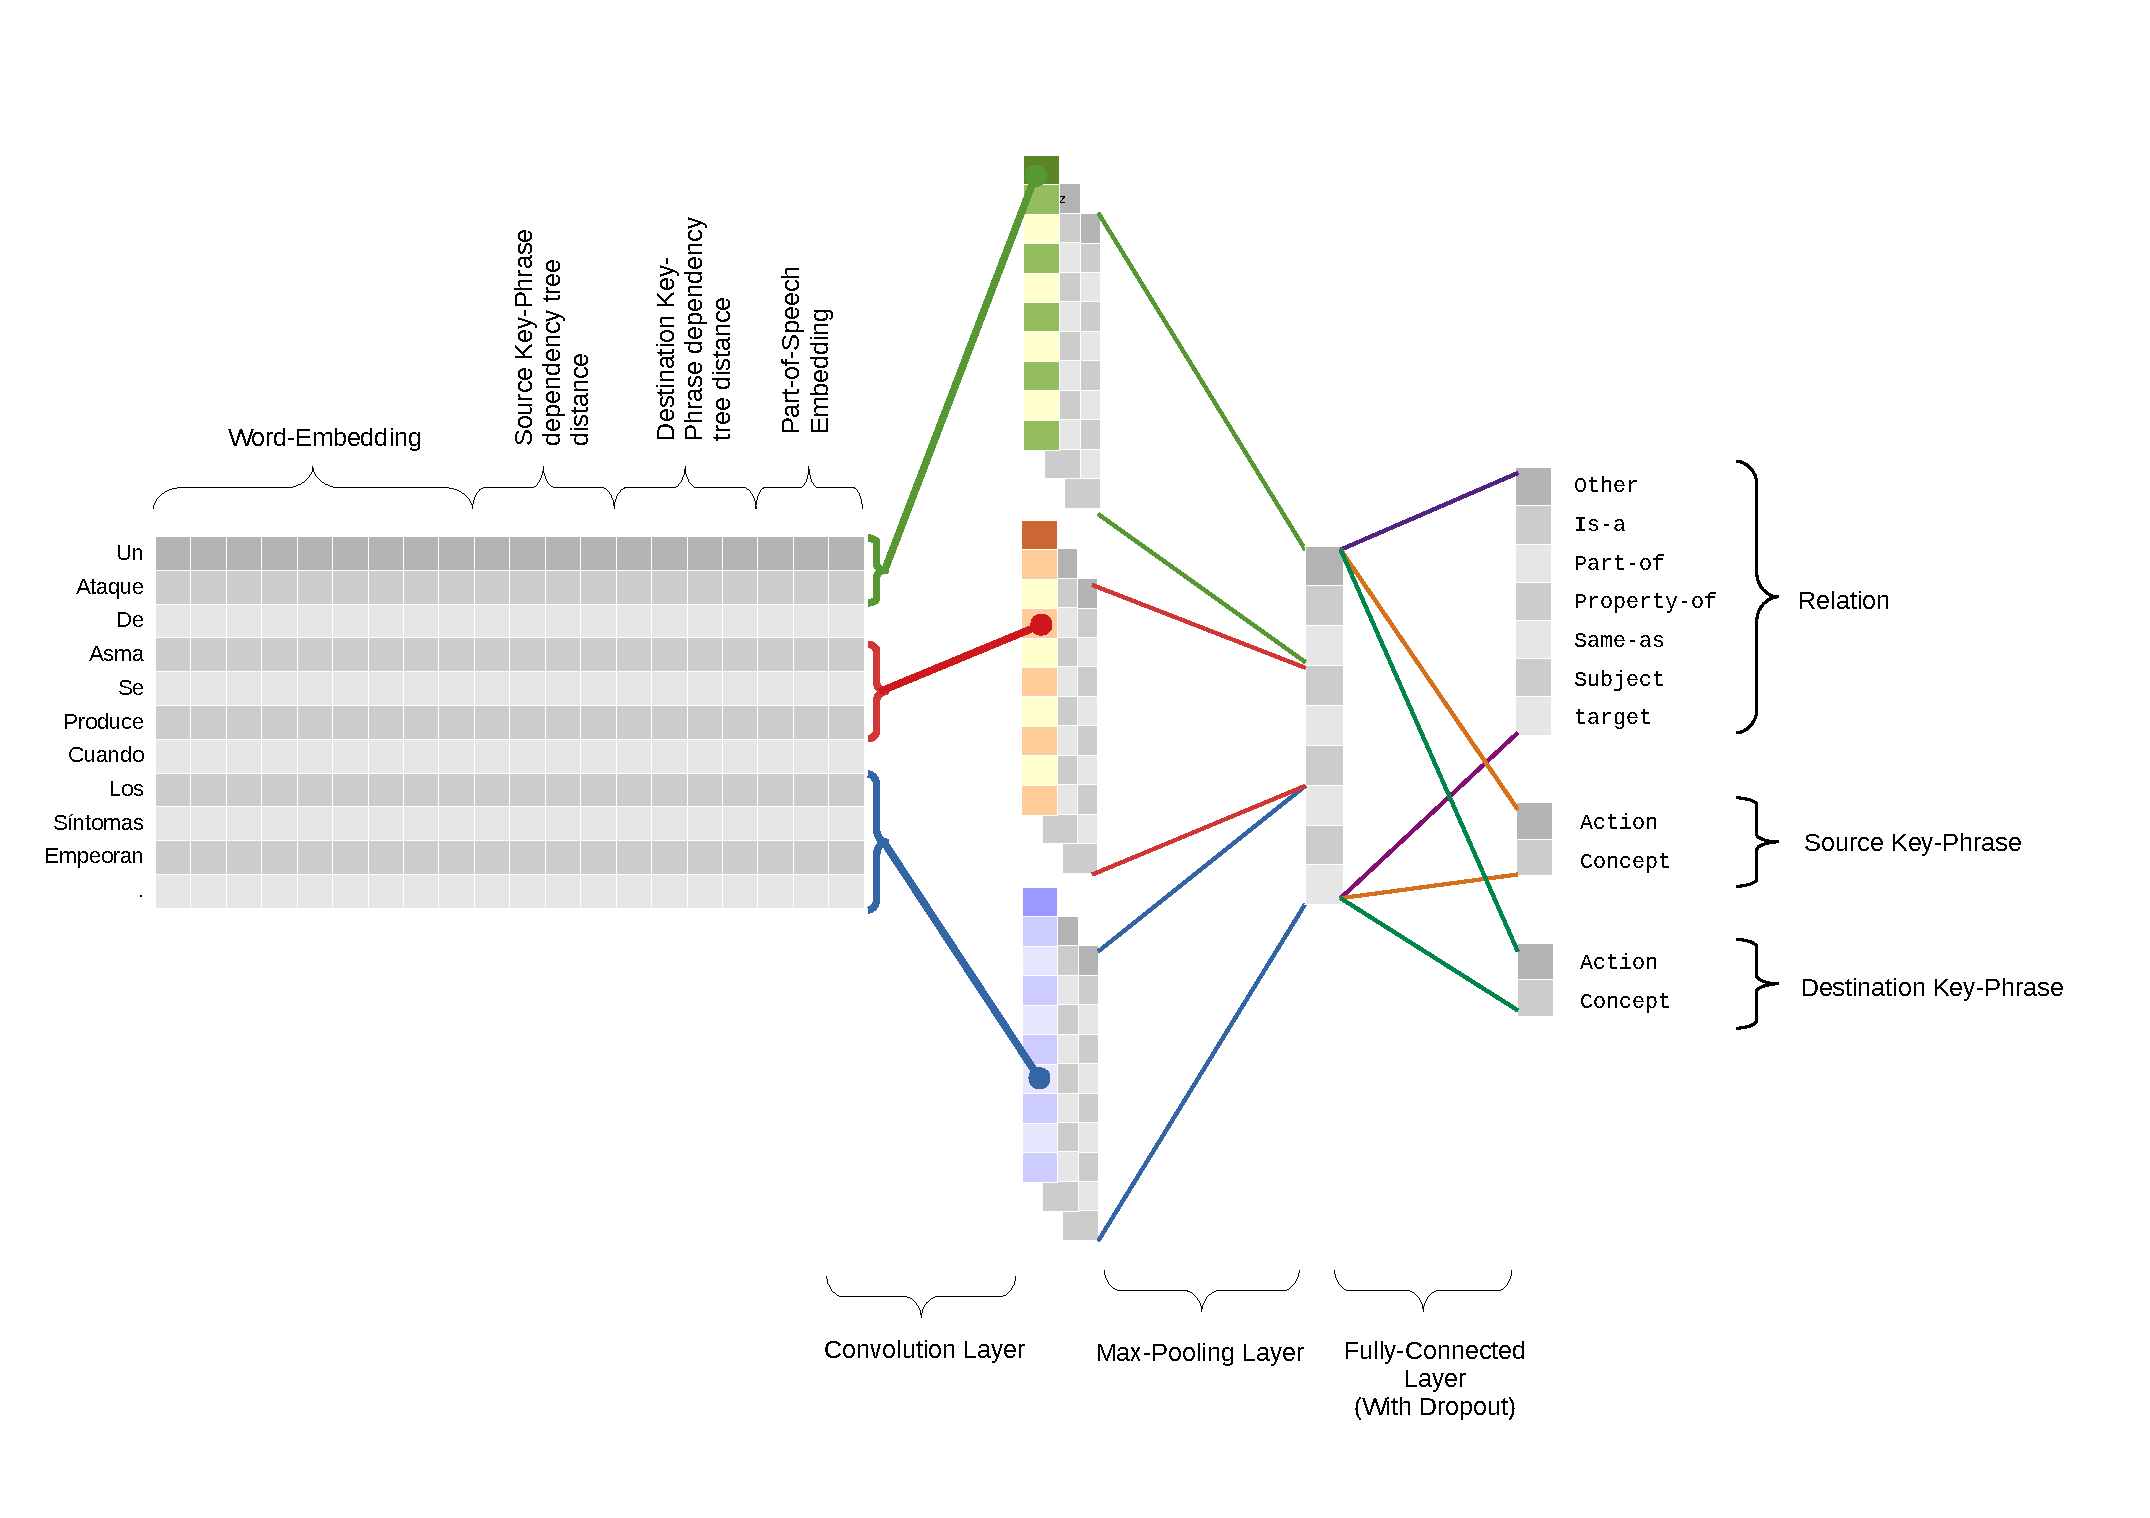
\includegraphics[width=0.9\linewidth,trim={0 1.7cm 0 2.2cm},clip]{diagramtass18.pdf}
    \caption{Layout of the proposed Convolutional Neural Network architecture}
    \label{fig:architecture}
\end{figure*}

The architecture that we propose is represented in Figure \ref{fig:architecture} and consists of a two-layer Convolutional Neural Network (CNN) which takes a vectorial representation of the documents and the position of two key-phrases as input and applies several convolution filters for window sizes from 1 to 4 tokens. The outputs of these filters are then max-pooled and fed to a fully connected output layer, which has two outputs for the given key-phrase pairwise: the probabilities of either key-phases for being \emph{Action} or \emph{Concept}, and the probabilities of the pairwise for being each possible kind of relationship, including \emph{``other''} for no relationship.


At first glance, our architecture is similar to the one proposed by the \emph{MIT} team for the \emph{ScienceIE} task, which also consists of a CNN using word-embedding, relative position and \emph{PoS-tags} as input features. However, it presents some noticeable differences. First of all, our architecture jointly tackles sub-tasks \emph{B} and \emph{C}.  For this reason, it does not take the key-phrase category as an input and has two additional outputs which hold the source and destination key-phrases' classes. Moreover, we optimize all three outputs at the same time and consequently our loss function is designed to reflect this.


\subsection{ Layout of the network and parameter optimization}

Artificial Neural Networks (ANN) and more specifically CNNs have proven to be capable of jointly identifying entities and relationships in various kinds of textual documents and relation extraction tasks, as it has been demonstrated in recent articles such as \cite{singh2013joint}, \cite{shickel2017deep} and \cite{li2017neural}. This joint identification takes advantage of the correlation that exists between linked entities aiming to provide better results for both named entity recognition classification and relation extraction tasks respect to a classical two-step system.

The loss function used by the parameter optimization algorithm is computed independently for the three outputs using soft-max cross-entropy, as classes are mutually exclusive for a single output, and is then combined by just adding the three losses. By adopting these three independent loss functions we can take profit of the fact that output classes for a single output are mutually exclusive and make their probabilities add up to one, independently of the other two outputs.

As for the optimization algorithm, we use \emph{TensorFlow's} \emph{Adam} optimizer with
a learning rate of $0.005$. The system was trained in batches of $128$ sentences
which were previously stripped to up to $50$ tokens and padded. We also apply a
\emph{dropout} rate of $0.5$ to the fully-connected output layer for regularization
purposes. The parameter optimization process is stopped either when the average \emph{loss} in the \emph{development} corpus remains flat for $1000$ iterations or when $1e5$ iterations have been run.


\subsection{Input parameters and encoding}

In order to come up with a manageable vectorial representation of the input sentences, they are
previously tokenized using \emph{FreeLing}'s with \emph{multi-word} and
\emph{quantity} detection as well as \emph{Named Entity Classification} (NEC)
modules disabled, so that multiple tokens are never joined together. These tokens are then
passed through a lookup table containing their pre-computed word-embeddings vectors, which are
then joined one-hot encodings of the relative positions respect to the target source
and destination key-phrases and their respective \emph{Part-of-Speech} (PoS) tag determined by
\emph{FreeLing}'s \emph{PoS-Tagger} module. A more detailed description of the input properties is listed below:

\begin{itemize}
\item \textbf{Word-Embedding}: 300-dimension vectorial representation of words in \emph{word2vec} format. We used the pre-trained general-purpose vectors from SBWCE \cite{cardellinoSBWCE}, trained from multiple sources.
\item \textbf{Distance to source or destination key-phrase}: One-hot encoding of the distance respect to the key-phrases. We consider two types of distances: absolute distance in terms of the number of tokens between each token and key-phrase and number of arcs in the dependency tree between each token and key-phrase, not taking into account the dependency class. The latter option was finally selected as it yielded better results in the validation corpus.
\item \textbf{Part-of-Speech tag}: One-hot encoding of the token's \emph{PoS-tag} determined by \emph{FreeLing}. For simplicity, we only contemplate the \emph{category} and \emph{type} positions of the \emph{PoS-tag}, hence reducing the number of different tags to 33.
\end{itemize}

\subsection{Data augmentation}

Relation extraction is a difficult task and usually requires big amounts of training examples in order to be able to correctly generalize the relationship classes. This is specially so for ANN based models, which can be prone to over-fitting. The training corpus that was provided for the \emph{TASS-2018} is very limited and classes are considerably unbalanced. To give an example, it only includes 30 instances of class \emph{same-as} compared to the 911 examples provided for class \emph{target}.

Because of this, we evaluated several data augmentation alternatives, which added slight modifications of the original training instances to the training set. These modifications included replacing some or all key-phrases by their class name or other key-phrases in the training corpus, or trimming the sentences removing some of their tokens. The alternative that worked best in the validation corpus and was used in the final model was to trim the context before and after the relationships to 1 and 3 tokens. For instance, in sentence  ``\emph{Un ataque de asma se produce cuando los síntomas empeoran.}'', the \emph{target} relationship between \emph{produce} and \emph{ataque de asma}, adds  ``\emph{Un ataque de asma se produce cuando}'' and  ``\emph{Un ataque de asma se produce cuando los síntomas}'', as well as the full sentence.

\section{Results}

\begin{table*}[ht]
    \centering
\begin{tabular}{r|cccccc|c}
\toprule
% \rotatebox{90}{Scenario} & \rotatebox{90}{plubeda} & \rotatebox{90}{rriveraz} & \rotatebox{90}{upf\_upc} & \rotatebox{90}{TALP} & \rotatebox{90}{VSP} & \rotatebox{90}{baseline} & \rotatebox{90}{Marcelo} \\
Scenario & plubeda & rriveraz & upf\_upc & VSP & baseline & Marcelo & TALP \\
\midrule
1 & 0.71 & \textbf{0.744} & 0.681 & 0.297 & 0.566 & 0.181 & N/A* \\
2 & 0.674 & 0.648 & 0.622 & 0.275 & 0.577 & 0.255 & \textbf{0.722} \\
3 & N/A* & N/A* & 0.036 & 0.42 & 0.107 & 0.018 & \textbf{0.448} \\
\bottomrule
avg & 0.461 & \textbf{0.464} & 0.446 & 0.331 & 0.417 & 0.151 & 0.39 \\
\end{tabular}
    \caption{Micro-averaged $F1$ score for evaluation scenarios 1 to 3 and global average. \emph{TALP} column shows our model's score. \textbf{N/A*}: Not Available, counted as 0 in the average score.}
    \label{tab:results}
\end{table*}

As it can be seen in Table \ref{tab:results}, our model scored first in the evaluation scenarios 2 and 3, which evaluate sub-tasks \emph{BC} and \emph{C} respectively. As it was mentioned in Section \ref{sec:introduction}, our system was designed for sub-tasks \emph{B} and \emph{C}, so no submission was sent for scenario 1, which also evaluates sub-task \emph{A}. In terms of the individual sub-tasks, our system raked first for sub-task \emph{C} but was outperformed by \emph{rriveraz}'s model in sub-task \emph{B}.


\subsection{Analysis of errors}

In this Subsection, we analyze the errors made by our model in \emph{Scenarios} \emph{2} and \emph{3}. Tables \ref{tab:confusion2a} and \ref{tab:confusion2b} show the confusion matrices for sub-tasks \emph{B} and \emph{C} in the evaluation of \emph{Scenario 2}. Results for sub-task \emph{C} in \emph{Scenario 3} are analogous to \emph{Scenario 2} and are not shown, as our model does not make use of the additional information given in \emph{Scenario 2}.


\begin{table}[t]
 \small
    \centering
\begin{tabular}{r|cc|c}
\toprule
true\textbackslash pred. & Concept &  Action & recall \\
\midrule
Concept &  \textbf{432} &       7 &  0.984\\
Action  &   34 &     \textbf{120} & 0.779\\
\bottomrule
precision & 0.927 & 0.945 & $Acc=0.931$


\end{tabular}
    \caption{Confusion matrix of our model's predictions for sub-task \emph{B} in scenario 2.}
    \label{tab:confusion2a}
\end{table}

\begin{table*}[ht]
\small
    \centering
    \begin{tabular}{r|ccccccc|c}
\toprule
 true\textbackslash pred. &  \rotatebox{90}{other} &  \rotatebox{90}{is-a} &  \rotatebox{90}{part-of} &  \rotatebox{90}{property-of} &  \rotatebox{90}{same-as} &  \rotatebox{90}{subject} &  \rotatebox{90}{target} & \rotatebox{90}{recall}\\
\midrule
other       &      \textbf{0} &     0 &        0 &            0 &        0 &        0 &       0 & 0.000 \\
is-a        &     31 &    \textbf{58} &        1 &            2 &        0 &        0 &       0 & 0.630 \\
part-of     &     26 &     2 &        \textbf{5} &            0 &        0 &        0 &       0 & 0.152 \\
property-of &     34 &     0 &        3 &           \textbf{18} &        0 &        0 &       3 & 0.310 \\
same-as     &      0 &     1 &        0 &            0 &        \textbf{0} &        0 &       0 & 0.000 \\
subject     &     65 &     0 &        0 &            2 &        0 &       \textbf{42} &       8 & 0.359 \\
target      &     84 &     0 &        1 &            7 &        0 &       12 &      \textbf{91} & 0.467 \\
\bottomrule
precision & 0.000 & 0.951 & 0.500 & 0.621 & 0.000 & 0.778 & 0.892 & $F_1=0.431$
\end{tabular}
    \caption{Confusion matrix, precision and recall of our model's predictions for sub-task \emph{C} in scenario 2. $F_1$ is micro-averaged for all classes.}
    \label{tab:confusion2b}
\end{table*}

% \subsubsection{Scenario 3}
%\begin{table}[]
%\footnotesize
%    \centering
%    \begin{tabular}{r|rrrrrrr}
%\toprule
%\rotatebox{90}{real\textbackslash predicted} &  \rotatebox{90}{other} &  \rotatebox{90}{is-a} &  \rotatebox{90}{part-of} & % \rotatebox{90}{property-of} &  \rotatebox{90}{same-as} &  \rotatebox{90}{subject} &  \rotatebox{90}{target} \\
%\midrule
%other       &      \textbf{0} &     0 &        0 &            0 &        0 &        0 &       0 \\
%is-a        &     31 &    \textbf{38} &        0 &            0 &        0 &        0 &       0 \\
%part-of     &     24 &     2 &        \textbf{3} &            2 &        0 &        1 &       0 \\
%property-of &     31 &     1 &        0 &           \textbf{27} &        0 &        1 &       2 \\
%same-as     &      4 &     0 &        1 &            0 &        \textbf{0} &        0 &       0 \\
%subject     &     77 &     0 &        1 &            3 &        0 &       \textbf{46} &      10 \\
%target      &     99 &     0 &        0 &            5 &        0 &       14 &      \textbf{94} \\
%\bottomrule
%\end{tabular}
%    \caption{Confusion table of our model's predictions for sub-task \emph{C} in scenario 3.}
%    \label{tab:confusion3}
%\end{table}

\subsubsection{Sub-Task B}
\label{sec:subtaskb}

Table \ref{tab:confusion2a} shows the confusion matrix for sub-task \emph{B} in \emph{Scenario 2}. Our model achieves similar \emph{precision} for classes \emph{Concept} and \emph{Action}, but \emph{recall} for the latter is 0.205 smaller. This is not only due to the fact that classes are unbalanced (439 and 154 instances of classes \emph{Concept} and \emph{Action} respectively), but also to other reasons listed below:

\begin{itemize}
    \item The \emph{Shared-Task's} description defines \emph{Actions} as a particular kind of \emph{Concept} that modifies another concept. Consequently, in some cases, the same phrase can either be an \emph{Action} or a \emph{Concept} depending on whether or not the modified \emph{Concept} is explicitly mentioned.
    As an illustration, the noun \emph{causa} (cause) is labeled as a \emph{Concept} in sentence ``\emph{El tratamiento depende de la causa.}'' (The threatment depends on the cause.). However, in sentence ``\emph{Es una causa común de sordera.}'' (It is a common cause of deafness.), it is labeled as \emph{Action}, as it is supposed to modify \emph{sordera} (deafness).
    \item Errors which were in part due to incorrect dependency parsing or \emph{PoS-tagging} by \emph{FreeLing}, specially when verbs are identified as nouns.
    
    For example, the noun \emph{oído} (ear) was identified as a verb in sentence ``\emph{Suele afectar sólo un oído.}'' (It usually affects just one ear.) by \emph{FreeLing}, which lead to confusion.
    Similarly, in sentence ``\emph{Esto causa una acumulación de sustancias grasosas en el bazo, hígado, pulmones, huesos y, a veces, en el cerebro.} (This causes an accumulation of fatty substances in the arm, liver, lungs, bones and, sometimes, the brain.), \emph{causa} (causes) is incorrectly labeled as a noun.
    \item Other instances where it is difficult to determine the label assigned to the entity, even for us, as they do not seem to correspond to any of the criteria exposed in the description. 
    
    For instance, in sentence ``\emph{Si usted ya tiene diabetes, el mejor momento para controlar su diabetes es antes de quedar embarazada.}'' (If you alredy have diabetes, the best moment to control your diabetes is before getting pregnant.), the adverb \emph{antes} (before) is labeled as \emph{Action} and is related to \emph{controlar} (control, keep) and \emph{quedar} (get, become) as \emph{subject} and \emph{target} respectively.
    
    On the other hand, in sentence ``\emph{La exposición al arsénico puede causar muchos problemas de salud.}'' (The exposition to arsenic can cause several health problems), the noun \emph{exposición} (exposition) is labeled as \emph{Concept}, while we understand it as the \emph{Action} of being exposed to something. This is not coherent to other instances such as ``\emph{No se conoce la causa de la destrucción celular.}'' (The cause of cell destruction is not known.), where \emph{destruction} is labeled as \emph{Action} - the \emph{Action} of being destroyed.
    \end{itemize}
    
\subsubsection{Sub-Task C}

\label{sec:subtaskc}

Table \ref{tab:confusion2b} shows the confusion matrix for sub-task \emph{C} in \emph{Scenario 2}. Class \emph{other} is used for all pairs of entities that have no specified relationship in the training set, making it the most frequent class in the training set. The model seems to prioritize \emph{precision} over \emph{recall}, which vary from class to class. Recall and precision for \emph{same-as}, although $0.000$, are not significant, as just one instance is present in the test set. The list below describes multiple reasons for the most common errors produced by our model:

\begin{itemize}
    \item Annotated instances in both training and test sets are unbalanced. Relationship counts in the training set range from 991 for \emph{target} and 693 for \emph{subject} to 149 and 30 for \emph{part-of} and \emph{same-as} respectively. What is more, the auxiliary class \emph{other} amounts to 16478 instances. More instances for the two less common classes seem to be required, as the model achieves much lower \emph{recall} and \emph{precision} than the most common ones.
    \item Relationships \emph{subject} and \emph{target} are prone to be mutually confused, specially for reflexive or passive verbs, and labeling is not always coherent. For example, in ``\emph{Algunos sarpullidos se desarrollan inmediatamente.}'' (Some skin rashes are developed immediately.), \emph{sarpullidos} (skin rashes) is \emph{subject} of \emph{se desarrollan} (are developed). However, in sentence ``\emph{Existen muchas razones para someterse a una cirugía.}'' (There are several reasons to have surgery.), \emph{razones} (reasons) is \emph{target} of \emph{existen} (there are).
    \item Multi-label relationships were not considered by our model, as we did not realize instances such as \emph{Durante cada trimestre, el feto crece y se desarrolla.} (During each quarter, the fetus grows and develops.), where the relationships between \emph{feto} (fetus) and \emph{crece} (grows), and similarly between \emph{feto} and \emph{se desarrolla} (develops), are both \emph{target} and \emph{subject}.
    \item Errors due to incorrect parsing by \emph{FreeLing}, which were already discussed in Section \ref{sec:subtaskb}.
\end{itemize}



\section{Conclusions and future work}

In this paper, we have described the model presented by the \emph{TALP} team for \emph{Task 3} of \emph{TASS-2018}. In addition we have presented some reasons for our model to wrongly classify key-phrases and relationships.

The results achieved by our model when compared to the rest of the challengers prove that a model that jointly classifies entities and relations can outperform traditional two-step systems in tasks where some entity classes are defined by the relationships they hold with others. There is however a big room for improvement, specially in the relation extraction task, mainly due to the increased complexity and the limited amount of examples available in the training set.

Our model was designed to solve the key-phrase classification and relation extraction tasks, leaving the key-phrase recognition as future work, as our focus was joint recognition and we did not have enough time to design and optimize a single model that could tackle all three tasks. We are committed to continue this line of investigation and extend the architecture so that it is also able to determine the key-phrases' boundaries.

Additionally, there are several improvements that could be applied to the current model, that we realized after analyzing the currently most common errors. To begin with, our model should allow for \emph{multi-label} relation extraction, as mentioned in Section \ref{sec:subtaskc}. Second, more syntactical features could be added, by for instance providing a complete and more appropriate encoding of the \emph{PoS-tags} or by including not only the dependency tree distances but also the types. 

% No sé como explicar que para identificar la clase de una key-phrase el modelo sólo mira a una de las relaciones con origen o destino esa key-phrase y no a todas las posibles
%% NO LO EXPLIQUES EN ESTE PAPER
\section*{Acknowledgments}
% JORDI: Ho acabo de ficar
This works has been partially funded by the Spanish Goverment and by the European Union through GRAPHMED project (TIN2016-77820-C3-3-R and AEI/FEDER,UE.)

\bibliographystyle{fullname}
\bibliography{main}

\end{document}